\documentclass[UTF8,12pt, a4paper]{ctexart}
\usepackage{geometry}
\usepackage{amsmath}
\usepackage{graphicx}
\usepackage{rotating}
\usepackage{arydshln}
\usepackage{color}
\usepackage[most]{tcolorbox}
\CTEXsetup[format={\large\bfseries}]{section}
% \usepackage{sectsty}
% \sectionfont{\fontsize{14}{15}\selectfont}
\usepackage{setspace}
\renewcommand{\baselinestretch}{1.5}
\geometry{left=2.0cm, right=1.5cm, top=2.5cm, bottom=2.5cm}
\title{Mechine Learning Assignment 1}
\author{}
\date{}
\begin{document}
  \maketitle
  \pagestyle{plain}
  \allowdisplaybreaks
  
\section{Generative and Discriminative classifiers: Gaussian Bayes and Logistic Regression} 
\noindent
Recall that a generative classifier estimates $P(x,y)=P(y)P(x|y)$, while a discriminative classifier directly estimates $P(y|x)$.
\subsection{Specific Gaussian naive Bayes classifiers and logistic regression} 

\noindent
Consider \textbf{a specific class} of Gaussian naive Bayes classifiers where:

\begin{itemize}
  \item $y$ is a boolean variable following a Bernoulli distribution, with parameter $\pi=P(y=1)$ and thus $P(y=0)=1-\pi$.
  \item $x=\left[x_1, ...,x_D\right]^T$ with each feature $x_i$ a continuous random variable. For each $x_i$, $P(x_i|y=k)$ is a Gaussian distribution $\mathcal{N}(\mu_{ik}, \sigma_i)$. Note that $\sigma_i$ is the standard deviation of the Gaussian distribution, which does not depend on $k$.
  \item For all $i \not= j$, $x_i$ and $x_j$ are conditionally independent given $y$ (so called “naive” classifier).
\end{itemize}
\textbf{\large{Question: }} 
please show that the relationship between a discriminative classifier (say logistic regression) and the above specific class of Gaussian naive Bayes classifiers is precisely the form used by logistic regression. \\
\begin{tcolorbox}[breakable, enhanced]
\textbf{\large{SOLUTION: }}\\
First of all, we can recall the expression of logistic regression as follow,
\begin{equation}
  P(y=1|x)= \frac{1}{1+\exp(w_0 + \sum_{i=1}^{D}{w_ix_i})}
  =\frac{1}{1+\exp(W^Tx)}.
\end{equation}
and with the definition of Gaussian distribution and Bernoulli distribution,
$$
\begin{aligned}
  y &\sim Bernoulli(\pi) \\
  x_i|y=k & \sim \mathcal{N}(\mu_{ik}, \sigma_i), k= \{ 0,1\} \\
\end{aligned}
$$
we can write the expression of each feature of $x$ and y,
\begin{align}
  P(y)&=\pi^k(1-\pi)^{1-y} \\
  P(x_i|y=k,\mu_{ik}, \sigma_i) &= \frac{1}{(2\pi\sigma_i ^2)^{1/2}} \exp\left(-\frac{(x_i-\mu_{ik})^2}{2\sigma_i^2}\right).
\end{align}
Because of our conditional independence assumption we can write this,
\begin{align}
    P(x|y=1) &= \Pi_{i=1}^{D}{P(x_i|y=1)}=\sum_{i=1}^{D}{\ln P(x_i|y=1)} \\
    P(x|y=0) &= \Pi_{i=0}^{D}{P(x_i|y=0)}=\sum_{i=1}^{D}{\ln P(x_i|y=0)}.
\end{align}
Now recall the Bayes' Forlula:
\begin{align}
  P(y|x)=\frac{P(x,y)}{P(x)}=\frac{P(x|y)P(y)}{P(x)},
\end{align}
we can compute a posterior probability of P(y=1|x), by \textbf{substituting eq.(4)(5) into eq.(6):}
\begin{equation}
  \begin{aligned}
    P(y=1|x)&=\frac{P(x|y=1)P(y=1)}{P(x|y=1)P(y=1)+ P(x|y=0)P(y=0)} \\
    & = \frac{1}{1+{\frac{P(x|y=0)P(y=0)}{P(x|y=1)P(y=1)}}}  \\
    & = \frac{1}{1+\exp\left\{ \ln \frac{P(x|y=0)P(y=0)}{P(x|y=1)P(y=1)}\right\}}  \\
    & = \frac{1}{1+\exp\left\{ \ln\frac{P(y=0)}{P(y=1)} +\ln \frac{P(x|y=0)}{P(x|y=1)}\right\}}  \\
    & = \frac{1}{1+\exp\left\{ \ln\frac{1-\pi}{\pi} +\sum_{i=1}^{D}\ln \frac{P(x_i|y=0, \mu_{i0}, \sigma_i)}{P(x_i|y=1, \mu_{i1}, \sigma_i)}\right\}} 
  \end{aligned}
\end{equation}
Now consider just the summation in the eq.(7), with the eq.(3) we can expand this term as follows:\\
\begin{equation}
  \begin{aligned}
    \sum_{i=1}^{D}\ln \frac{P(x_i|y=0,\mu_{i0}, \sigma_i)}{P(x_i|y=1,\mu_{i1}, \sigma_i)}
    &=\sum_{i=1}^{D}\ln \frac{
        \frac{1}{(2\pi\sigma_i ^2)^{1/2}} \exp\left(-\frac{(x_i-\mu_{i0})^2}{2\sigma_i^2}\right)
      }{
        \frac{1}{(2\pi\sigma_i ^2)^{1/2}} \exp\left(-\frac{(x_i-\mu_{i1})^2}{2\sigma_i^2}\right)
      } \\
      &=\sum_{i=1}^{D}\ln \exp \left\{
        \frac{
        (x_i-\mu_{i1})^2-(x_i-\mu_{i0})^2)
      }{
        2\sigma_i ^2
      }\right\} \\
      &=\sum_{i=1}^{D}\left\{
        \frac{
        (x_i-\mu_{i1})^2-(x_i-\mu_{i0})^2)
      }{
        2\sigma_i ^2
      }\right\} \\
      &=\sum_{i=1}^{D}\left\{
        \frac{
        (x_i^2 -2x_i\mu_{i1} + \mu_{i1}^{2})-(x_i^2 -2x_i\mu_{i0} + \mu_{i0}^{2})
      }{
        2\sigma_i ^2
      }\right\} \\
      &=\sum_{i=1}^{D}\left\{
        \frac{
        2x_i(\mu_{i0}-\mu_{i1}) + \mu_{i1}^{2} - \mu_{i0}^{2}
      }{
        2\sigma_i ^2
      }\right\} \\
      &=\sum_{i=1}^{D}\left\{
        \frac{(\mu_{i0}-\mu_{i1})}{\sigma_i ^2}x_i
        +\frac{ \mu_{i1}^{2} - \mu_{i0}^{2}}{2\sigma_i ^2}\right\}
  \end{aligned}
\end{equation}
So combine the result of eq.(7) and eq.(8), we can find that:
\begin{equation}
  \begin{aligned}
    P(y=1|x, \mu_{i0}, \mu_{i1}, \sigma_i)
    &=\frac{1}{1+\exp\left\{ \ln\frac{1-\pi}{\pi} + 
      \sum_{i=1}^{D}\left\{
      \frac{(\mu_{i0}-\mu_{i1})}{\sigma_i ^2}x_i
      +\frac{ \mu_{i1}^{2} - \mu_{i0}^{2}}{2\sigma_i ^2}\right\}  
      \right\}} \\
    &=\frac{1}{1+\exp(w_0 + \sum_{i=1}^{D}{w_ix_i})},
  \end{aligned}
\end{equation}
where the weight $w_1,...,w_D$ is given by
$$
w_i=\frac{\mu_{i0}-\mu_{i1}}{\sigma_i^2}
$$
and where
$$
w_i=\ln\frac{1-\pi}{\pi} 
  + \sum_{i=1}^{D}\left\{
   \frac{ \mu_{i1}^{2} - \mu_{i0}^{2}}{2\sigma_i ^2}
  \right\}
$$
Also we have the same form that
$$
P(y=0|x)=1-P(y=1|x) = \frac{\exp\left(w_0 + \sum_{i=1}^{D}{w_ix_i}\right)}{1+\exp\left(w_0 + \sum_{i=1}^{D}{w_ix_i}\right)}
$$
{\color{red}
So now we proved the relationship between a discriminative classifier and the above specific class of Gaussian naive Bayes classifiers is precisely the form used by logistic regression.\\
} 
\end{tcolorbox}

\subsection{General Gaussian naive Bayes classifiers and logistic regression}

Removing the assumption that the standard deviation $\sigma_i$ of $P(x_i|y=k)$ does not depend on $k$. That is, for each $x_i$, $P(x_i|y = k)$ is a Gaussian distribution $\mathcal{N}(\mu_{ik}, \sigma_{ik})$, where $i = 1,...,D$ and $k = 0,1$. \\
\textbf{\large{Question: }}is the new form of $P(y|x)$ implied by this more general Gaussian naive Bayes classifier still the form used by logistic regression? Derive the new form of$ P(y|x)$ to prove your answer. \\
\begin{tcolorbox}[breakable, enhanced]
\textbf{\large{SOLUTION: }} \\
As the assumption that the standard deviation $\sigma_i$ of $P(x_i|y=k)$ does not depend on $k$ is removed, we can rewrite the equations mentioned in the subsection 1.1.
Firstly, the definitions of general Gaussian naive Bayes classifiers are described as follows:
\begin{align}
  P(x_i|y=k,\mu_{ik}, \sigma_{ik}) = \frac{1}{(2\pi\sigma_{ik}^2)^{1/2}} \exp\left(-\frac{(x_i-\mu_{ik})^2}{2\sigma_{ik}^2}\right).
\end{align}
Also the posterior probability $P(y=1|x)$ of Bayes Formula can be rewritten as
\begin{equation}
  \begin{aligned}
    P(y=1|x)&=\frac{P(x|y=1)P(y=1)}{P(x|y=1)P(y=1)+ P(x|y=0)P(y=0)} \\
    & = \frac{1}{1+\exp\left\{ \ln\frac{1-\pi}{\pi} +\sum_{i=1}^{D}\ln \frac{P(x_i|y=0, \mu_{i0}, \sigma_{ik})}{P(x_i|y=1, \mu_{i1}, \sigma_{ik})}\right\}}  \\
  \end{aligned}
\end{equation}
so now we can substitute the equation(10) into the summation function in the equation(11),
\begin{align*}
    &\sum_{i=1}^{D}\ln \frac{P(x_i|y=0,\mu_{i0}, \sigma_{i0})}{P(x_i|y=1,\mu_{i1}, \sigma_{i1})} \\
    &=\sum_{i=1}^{D}\ln \frac{
        \frac{1}{(2\pi\sigma_{i0}^2)^{1/2}} \exp\left(-\frac{(x_i-\mu_{i0})^2}{2\sigma_{i0}^2}\right)
      }{
        \frac{1}{(2\pi\sigma_{i1}^2)^{1/2}} \exp\left(-\frac{(x_i-\mu_{i1})^2}{2\sigma_{i1}^2}\right)
      } \\
      &=\sum_{i=1}^{D}\ln \left\{ \frac{|\sigma_{i1}|}{|\sigma_{i0}|} \exp \left(
        \frac{(x_i-\mu_{i1})^2}{2\sigma_{i1} ^2}
        - \frac{(x_i-\mu_{i0})^2)}{2\sigma_{i0} ^2}
      \right) \right\}\\
      &=\sum_{i=1}^{D}\left\{
        \ln \frac{|\sigma_{i1}|}{|\sigma_{i0}|}
        + \frac{(x_i-\mu_{i1})^2}{2\sigma_{i1} ^2}
        - \frac{(x_i-\mu_{i0})^2)}{2\sigma_{i0} ^2}
      \right\} \\
      &=\sum_{i=1}^{D}\left\{
        \ln \frac{|\sigma_{i1}|}{|\sigma_{i0}|}
        +\frac{
         \sigma_{i0}^2 (x_i^2 -2x_i\mu_{i1} + \mu_{i1}^{2})
          - \sigma_{i1}^2 (x_i^2 -2x_i\mu_{i0} + \mu_{i0}^{2})
        }{
        4\sigma_{i1}^2\sigma_{i0}^2
        }\right\} \\
      &=\sum_{i=1}^{D}\left\{
        \ln \frac{|\sigma_{i1}|}{|\sigma_{i0}|}
        + \frac{\sigma_{i0}^2-\sigma_{i1}^2}{4\sigma_{i1}^2\sigma_{i0}^2}x_i^2
        + \frac{\sigma_{i1}^2\mu_{i0}-\sigma_{i0}^2\mu_{i1}}{2\sigma_{i1}^2\sigma_{i0}^2}x_i
        + \frac{\sigma_{i1}^2\mu_{i0}^2-\sigma_{i0}^2\mu_{i1}^2}{4\sigma_{i1}^2\sigma_{i0}^2}
        \right\}
\end{align*}
Now when substituting the equation above into the eq.(11), we get the form of general Gaussian naive Bayes classifiers as follow:
\begin{equation}
  \begin{aligned}
    P(y=1|x) & = \frac{1}{1+\exp\left\{ \ln\frac{1-\pi}{\pi} 
    + \sum_{i=1}^{D}\left\{
      \ln \frac{|\sigma_{i1}|}{|\sigma_{i0}|}
      + \frac{\sigma_{i0}^2-\sigma_{i1}^2}{4\sigma_{i1}^2\sigma_{i0}^2}x_i^2
      + \frac{\sigma_{i1}^2\mu_{i0}-\sigma_{i0}^2\mu_{i1}}{2\sigma_{i1}^2\sigma_{i0}^2}x_i
      + \frac{\sigma_{i1}^2\mu_{i0}^2-\sigma_{i0}^2\mu_{i1}^2}{4\sigma_{i1}^2\sigma_{i0}^2}
      \right\}
    \right\}}  \\
  \end{aligned}
\end{equation}
So the form of the classifiers is
\begin{equation}
  \begin{aligned}
    P(y=1|x) & = \frac{1}{1+\exp\left\{
      w_0
      + \sum_{i=1}^{D}{(w_ix_i + v_ix_i^2)}
    \right\}}  \\
  \end{aligned}
\end{equation}
where
\begin{align*}
  w_0 &= \ln\frac{1-\pi}{\pi}+ \sum_{i=1}^D{\ln\frac{|\sigma_{i1}|}{|\sigma_{i0}|} 
  +\frac{\sigma_{i1}^2\mu_{i0}^2-\sigma_{i0}^2\mu_{i1}^2}{4\sigma_{i1}^2\sigma_{i0}^2}}\\
  w_i &= \sum_{i=1}^{D}{\frac{\sigma_{i1}^2\mu_{i0}-\sigma_{i0}^2\mu_{i1}}{2\sigma_{i1}^2\sigma_{i0}^2}}\\
  v_i &= \sum_{i=1}^{D}{\frac{\sigma_{i0}^2-\sigma_{i1}^2}{4\sigma_{i1}^2\sigma_{i0}^2}} 
\end{align*}
Also we can get the similar for of the another posterior probability as this
\begin{equation}
  \begin{aligned}
    P(y=1|x) & = \frac{\sum_{i=1}^{D}{(w_ix_i + v_ix_i^2)}}{1+\exp\left\{
      w_0
      + \sum_{i=1}^{D}{(w_ix_i + v_ix_i^2)}
    \right\}}  
  \end{aligned}
\end{equation}
{\color{red} So we can get a conclusion that the new form of $P(y|x)$ implied by this more general Gaussian naive Bayes classifier {\color{black}\textbf{is not}} the form used by logistic regression,
and it can be written as the follow:
}
\begin{equation}
  \begin{aligned}
    P(y=1|x) & = \frac{1}{1+\exp\left\{
      w_0
      + \sum_{i=1}^{D}{(w_ix_i + v_ix_i^2)}
    \right\}}  \\
  \end{aligned}
\end{equation}
\begin{equation}
  \begin{aligned}
    P(y=0|x) & = \frac{\exp\left\{
      w_0
      + \sum_{i=1}^{D}{(w_ix_i + v_ix_i^2)}
    \right\}
    }{1+\exp\left\{
      w_0
      + \sum_{i=1}^{D}{(w_ix_i + v_ix_i^2)}
    \right\}}  \\
  \end{aligned}
\end{equation}
\end{tcolorbox}

\subsection{Gaussian Bayes classifiers and logistic regression}
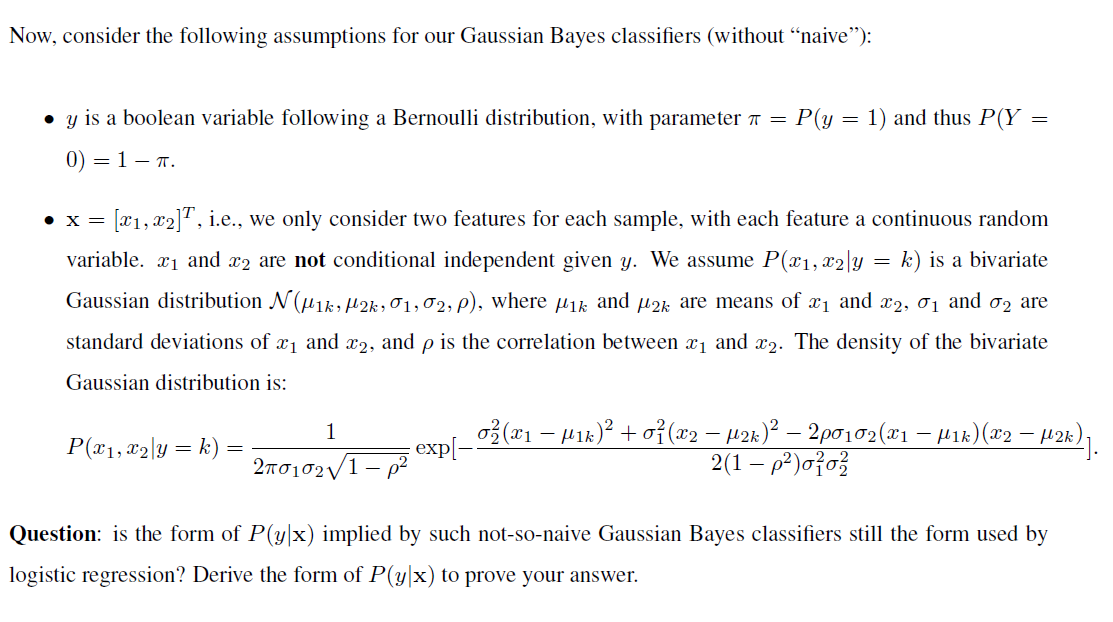
\includegraphics[scale=0.9]{question3.png} \\
\begin{tcolorbox}[breakable, enhanced]
\textbf{\large{Solution: }} 
Recall the Bayes Formula again and we have,
\begin{equation}
  \begin{aligned}
    P(y=1|x)&=\frac{P(x|y=1)P(y=1)}{P(x|y=1)P(y=1)+ P(x|y=0)P(y=0)} \\
    & = \frac{1}{1+{\frac{P(x|y=0)P(y=0)}{P(x|y=1)P(y=1)}}}  \\
    & = \frac{1}{1+\exp\left\{ \ln\frac{1-\pi}{\pi} +\ln \frac{P(x|y=0)}{P(x|y=1)}\right\}}.  \\
    \end{aligned}
\end{equation}
As described in the question, the density of the bivariate Gaussian distribution is:
\begin{align}
  P(x_1,x_2|y=k)
  =\frac{1}{2\pi\sigma_1\sigma_2\sqrt{1-\rho^2}}
  \exp\left\{
    -\frac{
      \sigma_2^2(x_1-\mu_{1k})^2
      + \sigma_1^2(x_2-\mu_{2k})^2
      - 2\rho\sigma_1\sigma_2(x_1-\mu_{1k})(x_2-\mu_{2k})
    }{
      2(1-\rho^2)\sigma_1^2\sigma_2^2
    }
  \right\}.
\end{align}
So we can substitute the equation (18) into the $ln$ function in equation (17), 
\begin{align*}
  &\ln \frac{P(x|y=0)}{P(x|y=1)} 
  = \ln \frac{P(x_1,x_2|y=0)}{P(x_1,x_2|y=1)} \\
  &=ln\left\{
    \frac{
      \frac{1}{2\pi\sigma_1\sigma_2\sqrt{1-\rho^2}}
      \exp\left\{
        -\frac{
          \sigma_2^2(x_1-\mu_{10})^2
          + \sigma_1^2(x_2-\mu_{20})^2
          - 2\rho\sigma_1\sigma_2(x_1-\mu_{10})(x_2-\mu_{20})
        }{
          2(1-\rho^2)\sigma_1^2\sigma_2^2
        }
      \right\}
    }{
      \frac{1}{2\pi\sigma_1\sigma_2\sqrt{1-\rho^2}}
      \exp\left\{
        -\frac{
          \sigma_2^2(x_1-\mu_{11})^2
          + \sigma_1^2(x_2-\mu_{21})^2
          - 2\rho\sigma_1\sigma_2(x_1-\mu_{11})(x_2-\mu_{21})
        }{
          2(1-\rho^2)\sigma_1^2\sigma_2^2
        }
      \right\}
    }
  \right\} \\
  &=ln\left\{
    \frac{
      \exp\left\{
        -\frac{
          \sigma_2^2(x_1-\mu_{10})^2
          + \sigma_1^2(x_2-\mu_{20})^2
          - 2\rho\sigma_1\sigma_2(x_1-\mu_{10})(x_2-\mu_{20})
        }{
          2(1-\rho^2)\sigma_1^2\sigma_2^2
        }
      \right\}
    }{
      \exp\left\{
        -\frac{
          \sigma_2^2(x_1-\mu_{11})^2
          + \sigma_1^2(x_2-\mu_{21})^2
          - 2\rho\sigma_1\sigma_2(x_1-\mu_{11})(x_2-\mu_{21})
        }{
          2(1-\rho^2)\sigma_1^2\sigma_2^2
        }
      \right\}
    }
  \right\} \\
  & \begin{aligned}
    =&\frac{
      \sigma_2^2(x_1-\mu_{11})^2
      + \sigma_1^2(x_2-\mu_{21})^2
      - 2\rho\sigma_1\sigma_2(x_1-\mu_{11})(x_2-\mu_{21})
    }{
      2(1-\rho^2)\sigma_1^2\sigma_2^2
    } \\
    &- 
    \frac{
      \sigma_2^2(x_1-\mu_{10})^2
      + \sigma_1^2(x_2-\mu_{20})^2
      - 2\rho\sigma_1\sigma_2(x_1-\mu_{10})(x_2-\mu_{20})
    }{
      2(1-\rho^2)\sigma_1^2\sigma_2^2
    }
  \end{aligned} \\
  & \begin{aligned}
    =&\frac{
      \sigma_2^2(x_1^2 -2x_1\mu_{11} + \mu_{11}^2 - x_1^2 + 2x_1\mu_{10} - \mu_{10}^2)
    }{
      2(1-\rho^2)\sigma_1^2\sigma_2^2
    } \\
    &+
    \frac{
      \sigma_1^2(x_2^2 - x_2\mu_{21} + \mu_{21}^2 - x_2^2 + x_2\mu_{20} - \mu_{20}^2)
    }{
      2(1-\rho^2)\sigma_1^2\sigma_2^2
    } \\
    & +
    \frac{
      2\rho\sigma_1\sigma_2(x_1x_2 - x_2\mu_{10} - x_1\mu_{20} + \mu_{10}\mu_{20}
      - x_1x_2 + x_2\mu_{11} + x_1\mu_{21} - \mu_{11}\mu_{21})
    }{
      2(1-\rho^2)\sigma_1^2\sigma_2^2
    }
  \end{aligned} \\
  & \begin{aligned}
    =&
    \frac{
      2 \sigma_2^2(\mu_{10} - \mu_{11})
      + 2\rho\sigma_1\sigma_2(\mu_{21}-\mu_{20})
    }{
      2(1-\rho^2)\sigma_1^2\sigma_2^2
    } x_1 \\
    &+
    \frac{
      2 \sigma_1^2(\mu_{20} - \mu_{21})
      + 2\rho\sigma_1\sigma_2(\mu_{11}-\mu_{10})
    }{
      2(1-\rho^2)\sigma_1^2\sigma_2^2
    } x_2 \\
    & +
    \frac{
      \sigma_2^2(\mu_{11}^2 - \mu_{10}^2)
      + \sigma_1^2(\mu_{21}^2 - \mu_{20}^2)
      + 2\rho\sigma_1\sigma_2(\mu_{10}\mu_{20}-\mu_{11}\mu_{21})
    }{
      2(1-\rho^2)\sigma_1^2\sigma_2^2
    }
  \end{aligned}
\end{align*}
So now we can get the complete form of the equation (17) as follow:
\begin{align}
  P(y=1|x_1,x_2)=\frac{
    1
  }{
    1+
    \exp\left\{
      w_0+ w_1x_1 + w_2x_2
    \right\}
  }
\end{align}
where,
\begin{align*}
  &w_2 = 
  \frac{
      2 \sigma_1^2(\mu_{20} - \mu_{21})
      + 2\rho\sigma_1\sigma_2(\mu_{11}-\mu_{10})
    }{
      2(1-\rho^2)\sigma_1^2\sigma_2^2
  } \\
  &w_1 = 
  \frac{
    2 \sigma_2^2(\mu_{10} - \mu_{11})
    + 2\rho\sigma_1\sigma_2(\mu_{21}-\mu_{20})
  }{
    2(1-\rho^2)\sigma_1^2\sigma_2^2
  }\\
  &w_0 = 
  \ln \frac{
    1-\pi
  }{
    \pi
  } + 
  \frac{
    \sigma_2^2(\mu_{11}^2 - \mu_{10}^2)
    + \sigma_1^2(\mu_{21}^2 - \mu_{20}^2)
    + 2\rho\sigma_1\sigma_2(\mu_{10}\mu_{20}-\mu_{11}\mu_{21})
  }{
    2(1-\rho^2)\sigma_1^2\sigma_2^2
  }
\end{align*}
Also, we have the similar form that
\begin{align}
  P(y=1|x_1,x_2)=\frac{
    \exp\left\{
      w_0+ w_1x_1 + w_2x_2
    \right\}
  }{
    1+
    \exp\left\{
      w_0+ w_1x_1 + w_2x_2
    \right\}
  }.
\end{align}
{\color{red}So, we can find that the form of $P(y|x)$ implied by such not-so-naive Gaussian Bayes classifier still the form used by logistic regression.}
\end{tcolorbox}
\end{document}
